The primary objective of a Convolutional Neural Network (CNN) is to enable a computer to identify images and objects, making it ideal for image classification and object recognition tasks. 

CNNs are based on the biological processes in the human brain and its connectivity patterns resemble those of the human visual cortex. However, images are perceived differently by the human brain and a computer, with the latter interpreting images as arrays of numbers. As a result, CNNs are designed to work with two-dimensional image arrays, although they can also work with one-dimensional or three-dimensional arrays \cite{mlmastery}.

CNN is a variation of FNN \cite{Goodfellow-et-al-2016}.  It typically consists of an input layer, followed by multiple hidden layers, including several \textit{convolutional layers} and \textit{pooling layers}, and concluding with an output layer.

\setsecnumdepth{all}
\subsubsection{Convolutional Layer}

The convolutional layer's goal is to extract key features from the input image by passing a matrix known as a \textit{kernel} over the input image abstracted into a matrix \cite{mathworkscnn}.

\begin{figure}[h]
	\centering
    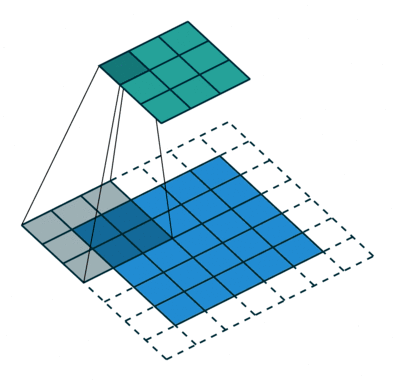
\includegraphics[width=8cm]{conv_layer_padding.png}
	\caption{Convolution of an 5x5x1 image with 3x3x1 kernel \cite{compguideCnn}}
	\label{fig:cnn_conv}
\end{figure}


The outcome of a convolution operation can be either reduced or increased in size. If the size is reduced, it is referred to as \textit{valid padding}. For example, a convolution operation on an 8x8 input image would result in a 6x6 convoluted feature. On the other hand, if the size remains the same or is increased, it is referred to as \textit{same padding} \cite{compguideCnn}.

\subsubsection{Pooling Layer}


Like the convolutional layer, the pooling layer reduces the size of the convolved feature to reduce computational power needed for data processing. It also extracts dominant features that are invariant to rotation and position, making it beneficial for training the model effectively \cite{compguideCnn}.

There are two types of pooling: max pooling and average pooling. Max pooling returns the maximum value from the portion of the image covered by the kernel, acting as a noise suppressant by removing noisy activations and performing de-noising and dimensionality reduction. Average pooling returns the average of all values in the same portion, reducing dimensions as a noise suppression mechanism. It is worth noting that max pooling performs better \cite{compguideCnn}.

\begin{figure}[h]
	\centering
    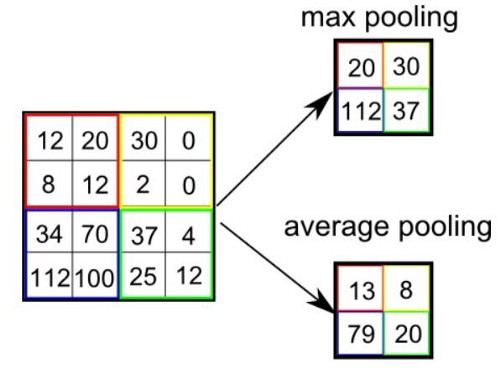
\includegraphics[width=8cm]{conv_pooling.png}
	\caption{Types of pooling \cite{compguideCnn}}
	\label{fig:cnn_pooling}
\end{figure}
